

\section{OpticalElement: \textquotedbl{}armazones\textquotedbl{}%
  \label{opticalelement-armazones}%
}

\textbf{Element}: atmosphere

\textbf{Alias}: ATMO

\textbf{Description}: Atmosphere and location details for Cerro Armazones


\subsection{Global properties%
  \label{global-properties}%
}

\begin{quote}
\begin{alltt}
\begin{lstlisting}[frame=single]
    altitude : 3060
   longitude : -70.1918
    latitude : -24.5899
 temperature : 7
    humidity : 0.1
    pressure : 0.755
         pwv : 2.5
     airmass : !OBS.airmass
 pupil_angle : !OBS.pupil_angle
 pixel_scale : !INST.pixel_scale
  background : \{'filter_name': 'Ks', 'value': 13.6, 'unit': 'mag'\}
    spectrum : \{'filename': 'TER_armazones_default_FULL_IMG.dat'\}
element_name : armazones
\end{lstlisting}
\end{alltt}
\end{quote}


\subsection{Effects%
  \label{effects}%
}

Summary of Effects included in this optical element:

\setlength{\DUtablewidth}{\linewidth}
\begin{longtable*}[c]{|p{0.114\DUtablewidth}|p{0.366\DUtablewidth}|p{0.246\DUtablewidth}|p{0.103\DUtablewidth}|p{0.125\DUtablewidth}|}
\hline
\textbf{%
element
} & \textbf{%
name
} & \textbf{%
class
} & \textbf{%
included
} & \textbf{%
z\_orders
} \\
\hline
\endfirsthead
\hline
\textbf{%
element
} & \textbf{%
name
} & \textbf{%
class
} & \textbf{%
included
} & \textbf{%
z\_orders
} \\
\hline
\endhead
\multicolumn{5}{c}{\hfill ... continued on next page} \\
\endfoot
\endlastfoot

armazones
 & 
armazones\_atmo\_default\_ter\_curve
 & 
AtmosphericTERCurve
 & 
True
 & 
{[}111, 511{]}
 \\
\hline

armazones
 & 
armazones\_atmo\_dispersion
 & 
AtmosphericDispersion
 & 
False
 & 
{[}231{]}
 \\
\hline

armazones
 & 
armazones\_atmo\_skycalc\_ter\_curve
 & 
SkycalcTERCurve
 & 
False
 & 
{[}112, 512{]}
 \\
\hline
\end{longtable*}
\label{tbl-armazones}


\subsubsection{AtmosphericTERCurve: \textquotedbl{}armazones\_atmo\_default\_ter\_curve\textquotedbl{}%
  \label{atmospherictercurve-armazones-atmo-default-ter-curve}%
}

\textbf{Included by default}: \texttt{True}

\textbf{File Description}: atmospheric emission and transmission

\textbf{Class Description}: <no docstring>

\textbf{Changes}:

\begin{itemize}
\item 2020-10-29 (MV) Created file
\end{itemize}


\paragraph{Data%
  \label{data}%
}

\begin{figure}[H]
\noindent\makebox[\linewidth][c]{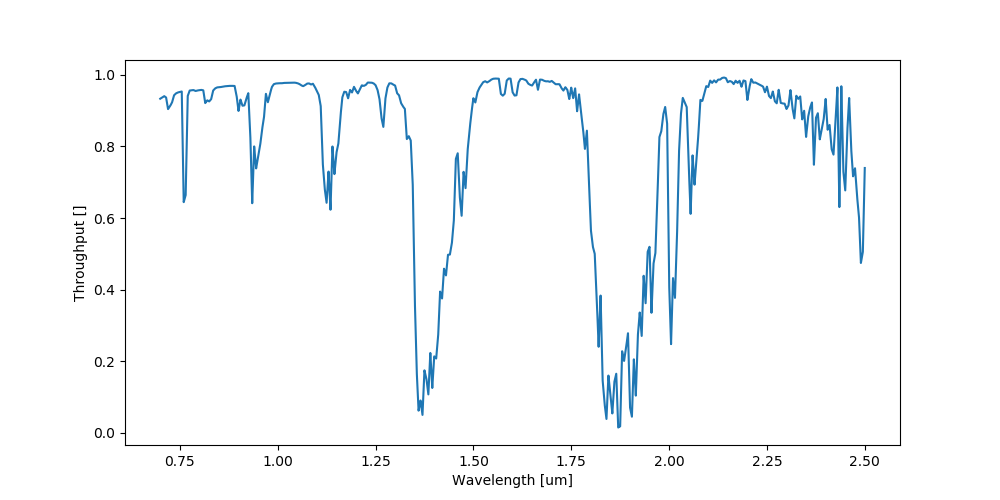
\includegraphics{armazones_atmo_default_ter_curve.png}}\phantomsection\label{fig-armazones-atmo-default-ter-curve}
\end{figure}


\paragraph{Meta-data%
  \label{meta-data}%
}

\begin{quote}
\begin{alltt}
\begin{lstlisting}[frame=single]
            filename : TER_armazones_default_FULL_IMG.dat
                name : armazones_atmo_default_ter_curve
             include : True
            altitude : 3060
           longitude : -70.1918
            latitude : -24.5899
         temperature : 7
            humidity : 0.1
            pressure : 0.755
                 pwv : 2.5
             airmass : 1.2
         pupil_angle : 0
         pixel_scale : 0.004
          background : \{'filter_name': 'Ks', 'value': 13.6, 'unit': 'mag'\}
            spectrum : \{'filename': 'TER_armazones_default_FULL_IMG.dat'\}
        element_name : armazones
                area : 0
    rescale_emission : \{'filter_name': 'Ks', 'filename_format': 'filters/TC_filter_\{\}.dat', 'value': 13.6, 'unit': 'mag'\}
              author : Miguel Verdugo
              source : skycalc_ipy tool for standard Armazones conditions
        date_created : 2020-10-29
       date_modified : 2020-10-29
              status : Design
                type : atmosphere:ter_curve
              wdelta : 10
                wmin : 300
                wmax : 15000
              season : entire year
                time : entire night
              action : transmission
     wavelength_unit : um
       emission_unit : ph s-1 m-2 um-1 arcsec-2
             z_order : [111, 511]
        ignore_wings : False
            wave_min : 0.7
            wave_max : 2.5
           wave_unit : um
            wave_bin : 0.0001
 report_plot_include : True
report_table_include : False
            position : 0
\end{lstlisting}
\end{alltt}
\end{quote}


\subsubsection{AtmosphericDispersion: \textquotedbl{}armazones\_atmo\_dispersion\textquotedbl{}%
  \label{atmosphericdispersion-armazones-atmo-dispersion}%
}

\textbf{Included by default}: \texttt{False}

\textbf{File Description}: atmospheric dispersion

\textbf{Class Description}: Used to generate the wavelength bins based on shifts due to the atmosphere

\textbf{Changes}:

\begin{itemize}
\item \end{itemize}


\paragraph{Data%
  \label{id1}%
}

\begin{figure}[H]
\noindent\makebox[\linewidth][c]{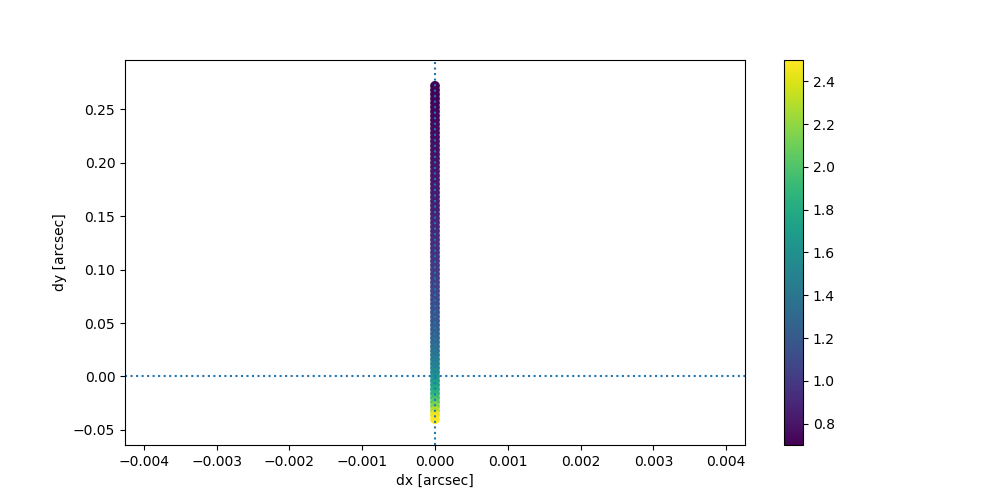
\includegraphics{armazones_atmo_dispersion.png}}\phantomsection\label{fig-armazones-atmo-dispersion}
\end{figure}


\paragraph{Meta-data%
  \label{id2}%
}

\begin{quote}
\begin{alltt}
\begin{lstlisting}[frame=single]
            filename : None
                name : armazones_atmo_dispersion
             include : False
            altitude : 3060
           longitude : -70.1918
            latitude : -24.5899
         temperature : 7
            humidity : 0.1
            pressure : 0.755
                 pwv : 2.5
             airmass : 1.2
         pupil_angle : 0
         pixel_scale : 0.004
          background : \{'filter_name': 'Ks', 'value': 13.6, 'unit': 'mag'\}
            spectrum : \{'filename': 'TER_armazones_default_FULL_IMG.dat'\}
        element_name : armazones
             z_order : [231]
 report_plot_include : True
report_table_include : False
            wave_min : 0.7
            wave_mid : 1.6
            wave_max : 2.5
  sub_pixel_fraction : 1
           num_steps : 1000
                  z0 : 33.55730976192071
                temp : 7
             rel_hum : 10.0
                pres : 755.0
                 lat : -24.5899
                   h : 3060
\end{lstlisting}
\end{alltt}
\end{quote}


\subsubsection{SkycalcTERCurve: \textquotedbl{}armazones\_atmo\_skycalc\_ter\_curve\textquotedbl{}%
  \label{skycalctercurve-armazones-atmo-skycalc-ter-curve}%
}

\textbf{Included by default}: \texttt{False}

\textbf{File Description}: atmospheric spectra pulled from the skycalc server

\textbf{Class Description}: <no docstring>

\textbf{Changes}:

\begin{itemize}
\item \end{itemize}


\paragraph{Data%
  \label{id3}%
}

\begin{figure}[H]
\noindent\makebox[\linewidth][c]{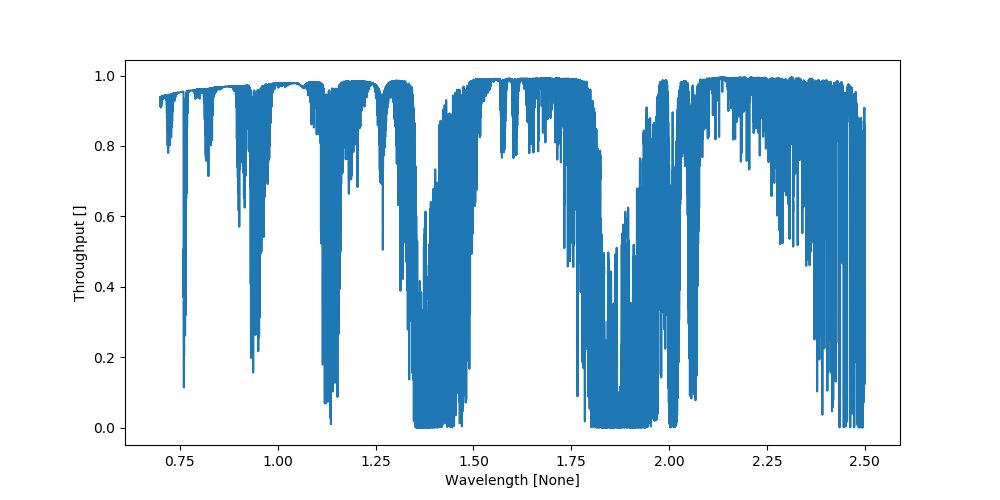
\includegraphics{armazones_atmo_skycalc_ter_curve.png}}\phantomsection\label{fig-armazones-atmo-skycalc-ter-curve}
\end{figure}


\paragraph{Meta-data%
  \label{id4}%
}

\begin{quote}
\begin{alltt}
\begin{lstlisting}[frame=single]
            filename : None
                name : armazones_atmo_skycalc_ter_curve
             include : False
            altitude : 3060
           longitude : -70.1918
            latitude : -24.5899
         temperature : 7
            humidity : 0.1
            pressure : 0.755
                 pwv : 2.5
             airmass : 1.2
         pupil_angle : 0
         pixel_scale : 0.004
          background : \{'filter_name': 'Ks', 'value': 13.6, 'unit': 'mag'\}
            spectrum : \{'filename': 'TER_armazones_default_FULL_IMG.dat'\}
        element_name : armazones
         observatory : armazones
                wmin : 699.9999999999999
                wmax : 2499.9999999999995
               wunit : um
              wdelta : 0.09999999999999999
             z_order : [112, 512]
        ignore_wings : False
            wave_min : 0.7
            wave_max : 2.5
           wave_unit : um
            wave_bin : 0.0001
 report_plot_include : True
report_table_include : False
              action : transmission
            position : 0
\end{lstlisting}
\end{alltt}
\end{quote}
